\section{The Delta Function}
In physics, we often consider the idea of a point mass. Suppose we have a unit point mass with mass density given by \(w(x)\). We are interested in the mass but do not know the details of its density. We do, however, know that the \(w(x)\) will be highly localized in space and that 
\begin{equation}
    \int_{-\infty}^{\infty} w(x) dx = 1
\end{equation}
so that the net force is unity.

We expect two highly concentrated mass densities to produce nearly identical masses except in the immediate neighborhood of the point at which the mass is concentrated. As such, we might simplify the problem by deciding, a priori, on a definite form for \(w\), such as
\begin{equation}
    w_k(x) = \begin{cases}
        \frac{k}{2}, & |x|<\frac{1}{k}\\
        0, & |x|>\frac{1}{k}
    \end{cases}
\end{equation}
or
\begin{equation}
    w_k(x)=\frac{k}{\pi (1+k^2x^2)}
\end{equation}
where \(k>0\). In Fig 3.2, we see that \(w\) becomes highly concentrated when \(k\) is large.

%Delta sequence diagram
\begin{figure}[H]
    \centering
    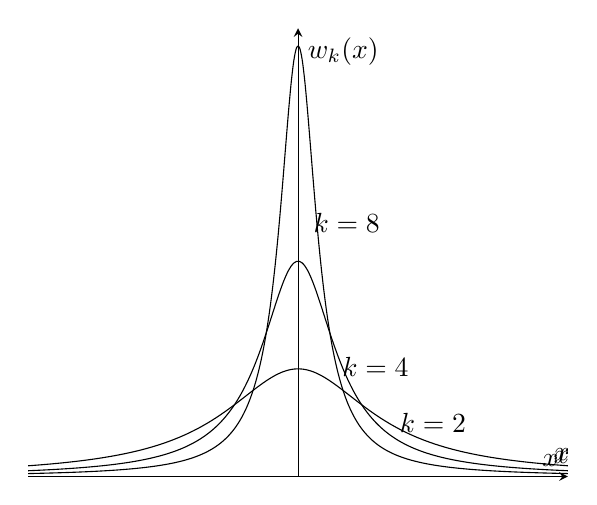
\begin{tikzpicture}
        \begin{axis}[
            axis lines = middle,
            xlabel = \(x\),
            ylabel = \(w_k(x)\),
            xtick = {0},
            ytick= {0},
            ymin=0,
            ymax = 2.65,
            restrict y to domain=0:2.65
        ]
            \addplot[
                samples=200, 
                smooth,
                domain = -1.5:1.5
                ] 
                {2/(pi*(1+2^2*x^2))};
                \node at (axis cs:0.75, 0.32) {$k=2$};
            \addplot[
                samples=200, 
                smooth,
                domain = -1.5:1.5
                ] 
                {4/(pi*(1+4^2*x^2))} node[above, pos=1]{$x^2$};
                \node at (axis cs:0.43, 0.65) {$k=4$};
            \addplot[
                samples=200, 
                smooth,
                domain = -1.5:1.5
                ] 
                {8/(pi*(1+8^2*x^2))} node[above, pos=1]{$x^2$};
                \node at (axis cs:0.27, 1.5) {$k=8$};
        \end{axis}
    \end{tikzpicture}
    \caption{Delta Sequence;  eq. 3.3}
\end{figure}

If we let \(k \rightarrow \infty\), then the force distribution approaches our idea of a "point-action," which in this case is a force of unit strength, acting at \(x=0\). Calling this "point-action" \(\delta(x)\), then
\begin{equation}
    \delta(x) = \lim_{k\rightarrow \infty} w_k(x)
\end{equation}
However, this cannot be considered a rigorous definition of the delta function because the limit is infinite for \(x=0\). 

\begin{definition}
    Generalized functions are continuous linear functionals that are continuous on the set of infinitely differentiable functions with compact support such that all generalized functions have derivatives which are also generalized functions.
\end{definition}

\begin{definition}
    A function has compact support if the subset of its domain for which its range is non-zero is closed and bounded.
\end{definition}

The delta function is more appropriately defined as a generalized function. To understand this way of defining \(\delta\), consider the following functional,
\begin{equation}
    \mathcal{F}(h) = \int_{-\infty}^{\infty} g(x)h(x).
\end{equation}
This functional assigns a numerical value, \(\mathcal{F}(h)\), for each function \(h\) within the domain, \(\mathcal{D}\), of \(\mathcal{F}\). We will take \(\mathcal{D}\) to be the set of all functions that are defined over \(-\infty <x<\infty\), are infinitely differentiable, and approach zero outside of some finite interval,

Suppose \(\mathcal{F}(h)\) is the integral of \(h\) from \(\xi\) to \(\infty\).
\begin{equation}
    \int_{\infty}^{\infty} g(x)h(x)dx = \int_{\xi}^{\infty} h(x) dx
\end{equation}
Then, \(g(x)\) must be the Heaviside step function,
\begin{equation}
    H(x) = \begin{cases}
        1, & x>0\\
        0, & x<0\\
        \frac{1}{2}, & x=0
    \end{cases}
\end{equation}
which is a function in the classical sense.

If \(\mathcal{F}(h)\) is \(h(0)\) so that
\begin{equation}
    \int_{-\infty}^{\infty}g(x)h(x) dx=h(0)
\end{equation}
then it can be shown that there is no function, \(g(x)\), which exists such that (3.8) is true for all functions, \(h(x)\), in the domain, \(\mathcal{D}\). It is then the case that \(g\) must be a generalized function, which we call the delta function. As such, \(\delta\) can be defined in the following way.
\begin{equation}
    \int_{-\infty}^{\infty} \delta(x)h(x) dx = h(0)
\end{equation}

Although \(\delta(x)\) acts at \(x=0\), it can be adjusted to act at any point by shifting the argument. Thus, \(\delta(x-\xi)\) acts at \(x=\xi\),
\begin{equation}
    \int_{-infty}^{\infty} \delta(x-\xi)h(x)dx = h(\xi)
\end{equation}
As a generalized function, \(\delta\) is also differentiable. By referring to (3.5), one can see that defining the derivative of a generalized function involves determining the functional, \(\mathcal{F}(h)\) for
\begin{equation}
    \int_{-\infty}^{\infty} g'(x)h(x) dx= \mathcal{F}(h)
\end{equation}
Next, we integrate by parts
\begin{equation}
    \intR g'(x)h(x)dx = g(x)h(x)\biggr\rvert_{-\infty}^{\infty} - \intR g(x)h'(x)dx
\end{equation}
The integral term is fairly simple to interpret since it is of the same form as (3.5), but the boundary term is not as nice because it involves knowing the values of \(g\). To deal with this, we will discard the boundary term and define \(g'\) with the formula
\begin{equation}
    \intR g'(x)h(x)dx = -\intR g(x)h'(x)dx
\end{equation}
For the delta function, this means
\begin{equation}
    \begin{split}
        \intR \delta'(x-\xi)h(x)dx &= -\intR\delta(x-\xi)h'(x)dx\\
        &=-h'(\xi)
    \end{split}
\end{equation}


\begin{theorem}
    The \(j\)th derivative of the delta function is defined by
    \begin{equation}
         \intR \delta^{(j)}(x-\xi)h(x)dx = (-1)^jh^{(j)}(\xi)
    \end{equation}
\end{theorem}
\begin{proof}
    By induction. I haven't figured out how to do this yet.
\end{proof}

Note that because of the discontinuity in \(H(x-\xi)\) at the point \(x=\xi\), the derivative of \(H\) does not exist as an ordinary function, but using the previous method does allow us to find \(H'(x-\xi)\) as a generalized function. 
\begin{equation}
    \begin{split}
        \intR H'(x-\xi)h(x)dx &= -\intR H(x-\xi)h'(x)dx\\
        &=-\int_{\xi}^{\infty}h'(x)dx = h(\xi)
    \end{split}
\end{equation}
and because
\begin{equation}
    \intR \delta(x-\xi)h(x)dx=h(\xi)
\end{equation}
it must be the case that
\begin{equation}
    H'(x-\xi) = \delta(x-\xi)
\end{equation}
Such equalities between generalized functions, as seen in (3.18), are understood in the sense that if some \(h\) in \(\mathcal{D}\) is multiplied through, and we integrate over \((-\infty, \infty)\) then the result will be consistent. That is to say
\begin{equation}
    \intR g_1(x)h(x)dx = \intR g_2(x)h(x)dx
\end{equation}
for some equivalent generalized functions \(g_1\) and \(g_2\).

As a final aside, notice that
\begin{equation}
    x\delta(x)=0
\end{equation}
as a result of
\begin{equation}
    \intR x\delta(x)h(x)dx=[xh(x)]|_{x=0} = 0
\end{equation}